\section{Seq2Seq ASR with Attention}

\begin{frame}[allowframebreaks]{Seq2Seq ASR with Attention}

\textbf{Encoder--Decoder Overview:}
\begin{itemize}
    \item \textbf{Encoder:} Processes the input acoustic features (e.g., Mel-spectrograms) and encodes them into a sequence of hidden representations.
    \item \textbf{Decoder:} Generates the output transcription, one token at a time, conditioned on the encoder outputs and previous decoder states.
    \item \textbf{Attention Mechanism:} Allows the decoder to focus on relevant parts of the input sequence at each decoding step, improving alignment and performance.
    \item Unlike CTC, nothing forces the alignment to be monotonic and no independence assumption is made across output tokens: the decoder is free to attend anywhere.
\end{itemize}

\framebreak

\textbf{Listen, Attend and Spell (LAS):} the canonical instance of this design.
\begin{itemize}
    \item The \textbf{listener} is a pyramidal BLSTM encoder that shortens the frame sequence $\mathbf{x}$ (length $T$) into $\mathbf{h}$ (length $U \leq T$).
    \item The \textbf{speller} is an attention-based decoder emitting characters $y_i$ one at a time.
\end{itemize}

\begin{figure}[h]
    \centering
    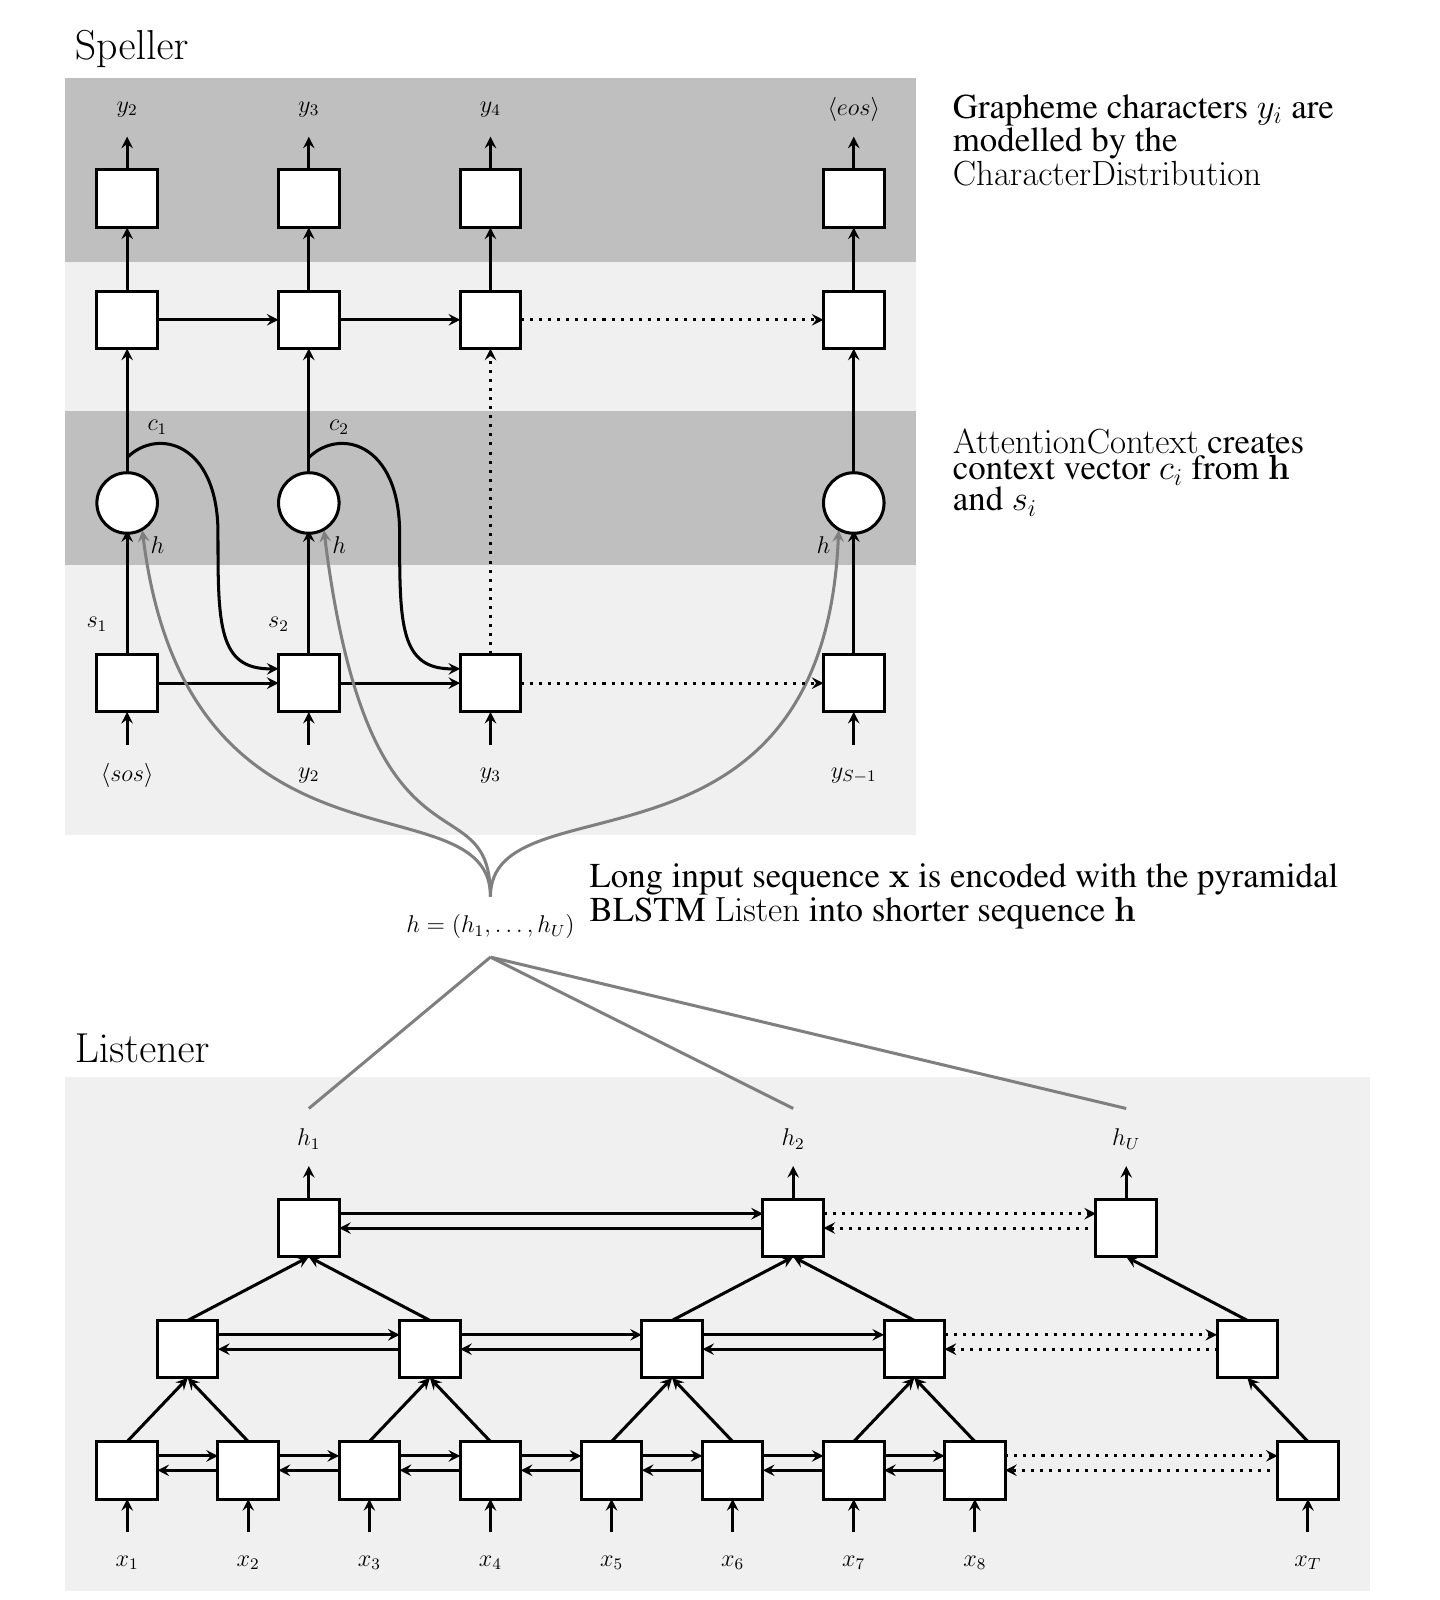
\includegraphics[width=\textwidth,height=0.62\textheight,keepaspectratio]{images/audio-nlp/las_architecture_chan2016.png}
    \caption*{\scriptsize Source: Chan et al., ``Listen, Attend and Spell'', ICASSP 2016, Fig.~1.}
\end{figure}

\framebreak

\textbf{Attention Alignment:}

At each decoder time step $t$, the attention mechanism computes a context vector as a weighted sum of encoder outputs. The weights $\alpha_{t,s}$ represent the alignment between decoder step $t$ and encoder position $s$:

\begin{equation}
    \alpha_{t,s} = \frac{\exp(e_{t,s})}{\sum_{s'} \exp(e_{t,s'})}
\end{equation}

where $e_{t,s}$ is the attention score (e.g., computed via a feedforward network) between decoder state at time $t$ and encoder output at position $s$.

\framebreak

\textbf{What the alignment looks like in practice}

\begin{itemize}
    \item Plotting $\alpha_{t,s}$ for every output character gives a heatmap of decoder step against audio frame.
    \item For speech it comes out close to diagonal, because speech is produced in order, even though nothing in the model enforces that.
    \item Where the model is unsure the mass spreads out: below, ``woodchuck'' draws a diluted band because ``woodchuck'' and ``chuck'' sound alike.
\end{itemize}

\begin{figure}[h]
    \centering
    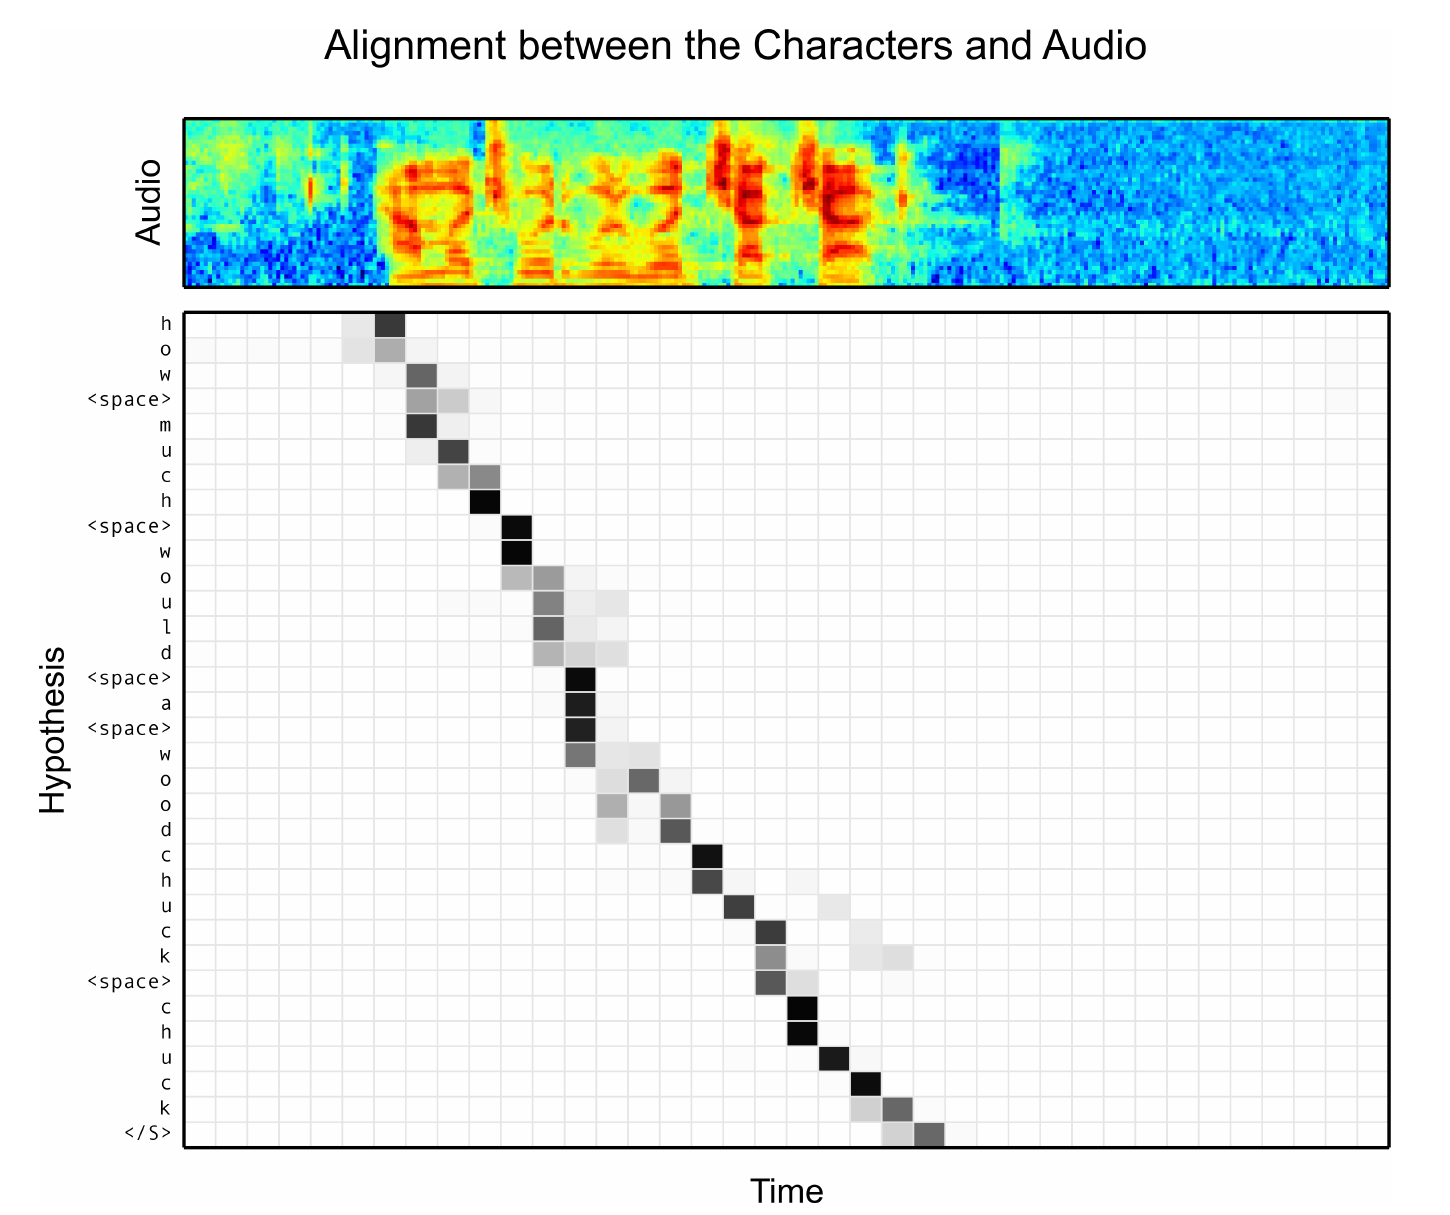
\includegraphics[width=\textwidth,height=0.6\textheight,keepaspectratio]{images/audio-nlp/las_attention_alignment_chan2016.png}
    \caption*{\scriptsize Alignment for the utterance ``how much would a woodchuck chuck''. Source: Chan et al., ``Listen, Attend and Spell'', ICASSP 2016, Fig.~2.}
\end{figure}

\end{frame}
